\chapter{Literature Review}
\label{chap:lr}
\chaptermark{Second Chapter Heading}

\section{Conventional compilers in the modern world}
\label{sec:review_1}

Since the middle of $20^{th}$ century researchers and the industry have done a great
work in compilers development focusing on the main goal of classic compilation
problem: producing fast and effective object code for execution on a virtual
machine or a microprocessor.


However, the other compilers` capability as developer`s code inspection
instruments able of providing comprehensive information of code semantics
remains uncommon and rarely well-developed in the modern compilers of
popular programming languages.


The most common illustration of this problem can be found in an average Java
developer`s set of instruments:

Java code is usually compiled with Sun Java Compiler. ``Being a
monolithic program, constructed as a `black box`"\cite{Zouev2005}, Sun Java Compiler can only accept the input
code and produce optimized JVM byte code.


Yet a modern development environment includes a set of tools for
programming assistance and requires advanced language syntax and
semantics inspection, which is not possible without building a Semantic
Representation\cite{Zouev2005}. To build it one needs to re-implement core functionality of a
compiler.


It`s easy to understand the very reason of the issue looking back to the past:
traditionally programs have been considered as mere text objects to be
converted into an executable code. According to this assumption, compilers
were designed in a very logical way: they haven`t maintained any semantic
representation of source code, only some low-level internal IR.


These compilers` IRs have very limited set of use cases\cite{Zouev2005, Zouev2010}, moreover they are
good for the only task: object code generation for several microprocessor
architectures. Also compiler`s IR is not stable and tends to change very actively
during compiler development\cite{FreeSoftwareFoundation2016}. Hence the internal compiler`s IR can`t really
be used to build good and reliable development tools.


The situation is even more frustrating with C++ tooling: the language syntax
and semantics is a lot more complicated than Java`s, so building a custom
compiler is a very complex task.

As a result, there is a notable lack of instruments for C++\cite{Zouev2010}, and existing
ones are pretty sophisticated: JetBrains CLion IDE implements its own parser
and semantic analyzer to build auto-completion, refactoring and static analysis
tools upon their own C++ SR. Being a complex software product, CLion`s parser
tends to have its own misfeatures and a few month implementational lag to
fully adapt for new standards.


Microsoft Visual Studio “suffers” from this too: VC++ generates IR that is useful
only for code generation: it is fragmented and very low-level.
The C\&C++ IntelliSense tooling in Microsoft Visual Studio IDE is implemented
as a solution separate from VC++ compiler.

\section{Modern compilers and SR: \\a new hope}
\label{sec:review_2}

In spite of the fact that traditional compilers are widely used today, their lack of
IDE integration capabilities were realized long ago and currently a lot of new
languages are aiming to implement a Semantic Representation as a stable IR
shared with external tools.

Following \cite{Zouev2005, Zouev2010}, unlike a traditional compiler IR, Semantic Representation contains a full
knowledge of a program, including the aspects that are implicit in the source
code. This trait enables some pretty powerful opportunities based on
semantics analysis:

\begin{itemize}
    \item Code generation
    \item Distributed (or recursive) Validation
    \item Human understandable visualization
    \item Static analysis
    \item Program interpretation
    \item Semantic Search: the very powerful technique of querying code semantic objects (“find all classes derived from class C that do not override the virtual function f”)
\end{itemize}

There are two main ways to represent an SR and share it with SR clients: to
provide an access API operating on an SR (proprietary) binary format \cite{Cannon, FreeSoftwareFoundation2016},
relational database representing a software structure \cite{Linton1983}, or to output SR as an
open textual format\cite{TheRustTeam2016}.

In accordance with \cite{Zouev2005},``Generally speaking, API is a universal way to implement any required
functionality, however with changing requirements it`s impossible to predict a
spectrum of clients` needs''.\\
And an open SP format can be a solution to potential problems: ``open formats
usually have a lot of access means: from simple APIs to high level specialized
products. Besides, it`s possible to implement one`s own interfaces to process SR
represented with open format''.

A particular format may be something self-designed[7] or a standardized
solution such as XML\cite{Germon}, or JSON\cite{ECMA-4042013}, as an alternative.

\newpage
\section{LSP and distributed approach to building development
environment}
\label{sec:review_3}

Considering the things discussed above, nowadays we have a solid basis to
provide a good tooling based on semantic analysis: methods to represent
software source code`s Semantic Representation and evaluate it accordingly to
clients` needs.

Modern IDEs apply those methods to deliver a decent service, but still there is a
problem: those software products use their own implementations of compilers,
usually proprietary and unrelated to the original language`s development team.
It implies a set of problems noted in the \ref{sec:review_1}.

Having a good modern compiler capable of generating an SR makes things a bit
less complicated but still doesn`t solve the language-specific IDE
implementation time and cost problem.

Obviously, these problems are not unique for the IDE class of products, but for
any big monolithic architecture, and the solution may be pretty straightforward:
if we can lower the bonding of the system and represent a development
environment as a set of tools instead of one integrated solution, we can
distribute the IDE implementation to have a set of disjointed modules:
\begin{itemize}
    \item An editor
    \item Compiler to SR
    \item SR clients (described in \ref{sec:review_1})
    \item Protocol between an editor and the language-specific part
\end{itemize}
\newpage

\begin{figure}[H]
    \centering
    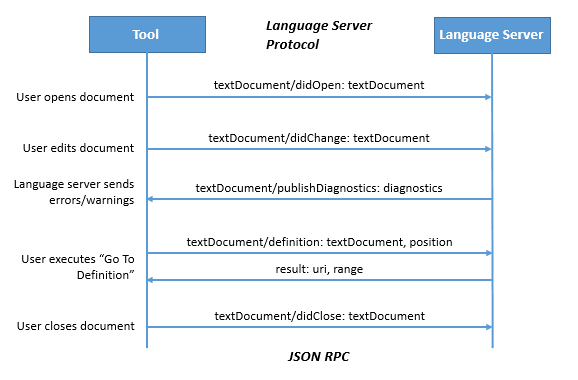
\includegraphics[width=0.85\textwidth]{figs/lsp.png}
    \caption{Language Server Protocol}
\end{figure}

The last one have not been introduced yet: the protocol to connect any
third-party tool to the language infrastructure, achieving a decent IDE-like
functionality without its maintenance and development costs

Language Server and Language Server Protocol introduced by Microsoft in 2016
represent a development environment as two disjoint parties:
\begin{itemize}
    \item Language Servers to implement all the SR analysis things
    \item Clients as editors or other development tools using the LSP to communicate with Language Servers \cite{Sourcegraph}
\end{itemize}

\section{Conclusion}
\label{sec:review_conclusion}

Conventional compilers with a monolithic architecture, that are only good at executable code generation,
are hard to integrate into a modern development environment as they do not share
semantic representation of the source code, thus to develop a good IDE one must write their own
source code to Semantic Representation compiler.

A modern compiler (that does share a high-level intermediate representation) is
a big step towards simpler language toolings and it can become even more convenient
combined with a distributed IDE architecture that splits an editor and the language toolchain
into two disjoint parts, linking them via a standardized protocol.

This approach gives language developers a great opportunity to make use of an
existing development infrastructure, providing their Language Server for a
giant set of development tools, as well as a way to fearlessly experiment with new and
existing analysis techniques, e.g. a Software Knowledge Base\cite{Wanghong}, described by
Bertrand Meyer, may be implemented as a language server module, as an
alternative approach to the one selected by the original author in 1985:
integration of analysis tool into an editor was not possible back then, but this is
the exact thing that LSP is good for now.

Concluding, the Language Server may be considered to be the most feasible
solution to rapidly bootstrap rich development infrastructure for aspiring new
languages, with a broad path to evolve further.